\chapter{Using a laboratory journal for better reproducibility}
\label{chapter:orgmode}

    Throughout the several years of this thesis, we used meticulously a laboratory journal, inspired by the lectures
    from Legrand~\etal~\cite{RR_mooc,SMPE_course}. Since we firmly believe that this was a great help for improving the
    reproducibility of this work, this chapter describes succintly our methodology.

    The journal is written with Org-mode~\cite{orgmode}. This is a mode from the Emacs text editor for editing,
    formatting and organizing text documents, using a lightweight markup language. It offers multiple functionnalities
    such as hierarchy within a file, TODO lists, tags, hyperlinks, file attachments and even code execution. We use git
    for versionning and collaborating.

    The journal follows a chronological order and hierarchy, as illustrated by
    Figure~\ref{fig:appendix:journal_extract}. There is one main part for each year, then subparts for months and days.
    Within the part of a given day, we create additional subparts, called \emph{journal entries}, related to the topic
    that should be recorded. Each part can be folded and unfolded to keep a reasonable amount of displayed text. For
    instance, in Figure~\ref{fig:appendix:journal_extract}, the first journal entry of 2021 is simply a link to a video
    presentation.

    Each journal entry can have one or several tags, displayed on the right in upper-case and delimited by colons. These
    key words are used for organizing the different entries by semantic. For instance, we can easily list all the
    entries related to experiments made on the dahu cluster by making a search for the tag \texttt{DAHU}.

    We used three kinds of journal entries:
    \begin{description}
        \item[Experiment analysis] All the experiments carried during this thesis have been executed by the Peanut
            experiment engine (see Part~\ref{part:experiment}), resulting in an archive containing data and meta-data
            for the experiment. Then, we collected, analyzed and made plots for these archives using literate
            programming, with Jupyter notebooks~\cite{jupyter}. Although this could be done directly within Org-mode,
            thanks to its code execution capability, we simply preferred the Jupyter ecosystem. When the analysis was
            done, we compiled the notebook to HTML, created a new entry in the journal and attached the notebook. This
            process has been automatized by a Python script we made, called \texttt{org\_attach}. This new entry
            contains at least two parts, one to summarize the experiment (what, why and how) and one to list the various
            observations we made in the analysis.
        \item[Paper reading] Whenever we find an interesting paper, we create a new journal entry, named after the paper
            title. The entry is marked with a keyword \texttt{READ} or \texttt{UNREAD} if we have already read the
            paper or not. The entry also contains at least three parts, namely the paper abstract, any notes we may have
            taken while reading the paper, and the bibtex. Finally, the PDF file of the paper is attached to the entry.
            Again, the process of creating the new entry and attaching the paper is automatized by \texttt{org\_attach}.
        \item[Free text] We also write in the journal any relevant material. This can be a discussion with colleagues,
            a seminar we attended, some unorganized thoughts, a short piece of code to test a new idea or demonstrate a
            new tool, etc. Again, the use of proper tags is important to be able to find these entries after a while.
    \end{description}
    \todo{Cite org\_attach}

    In the end, the text file of the journal has now more than one thousand entries. The text file has a size of more
    than \NSI{2.7}{\mega\byte}, while the attachments totalize more than \NSI{1.1}{\giga\byte}.

    \begin{figure}[htpb]
        \centering
        \fbox{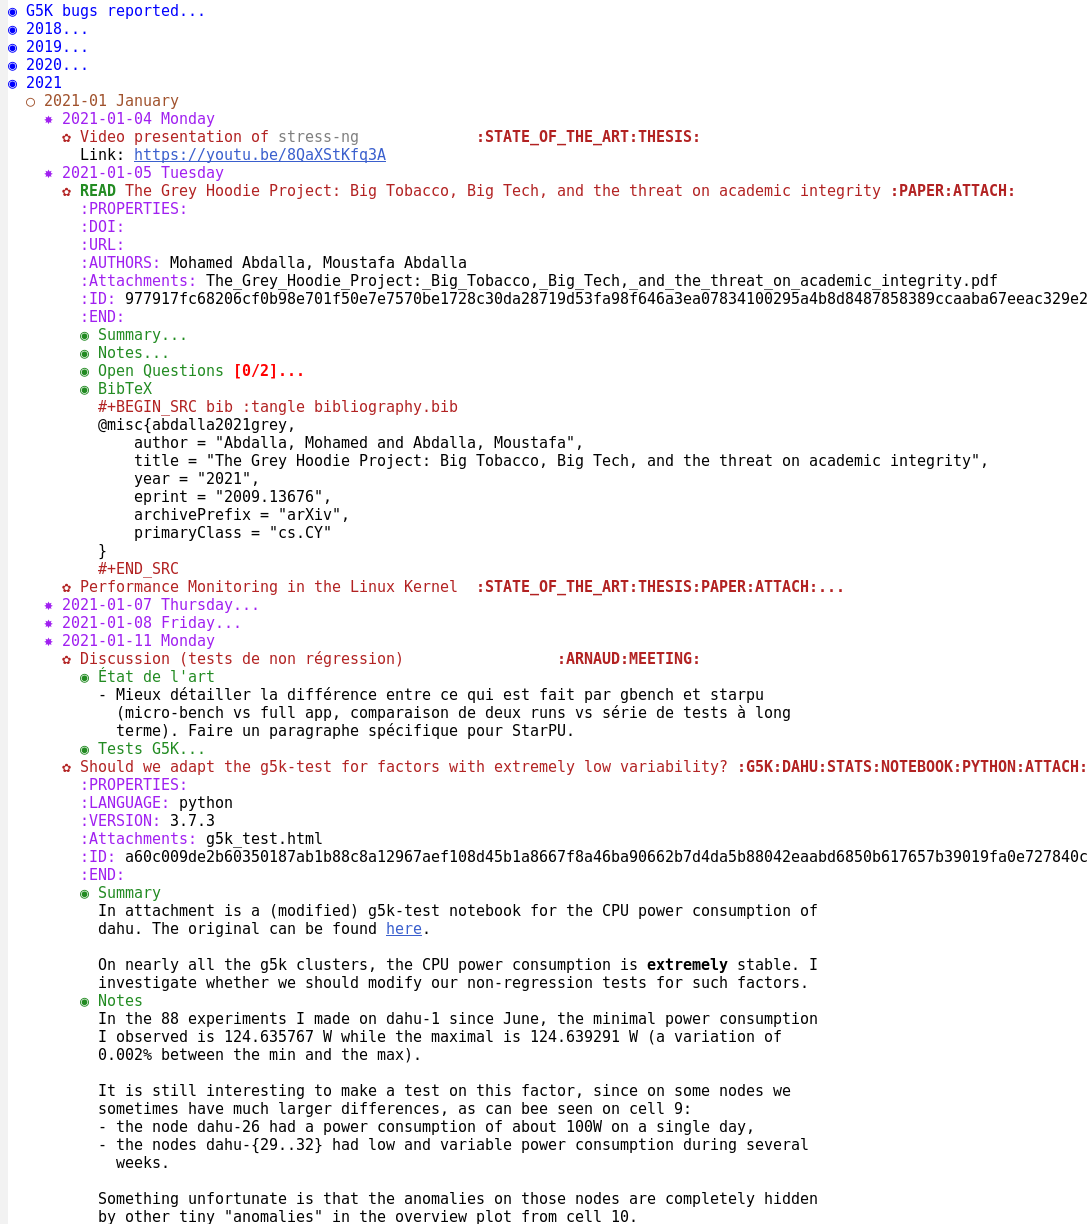
\includegraphics[width=\linewidth]{img/orgmode/journal_extract.png}}
        \caption{Screenshot of the laboratory journal used throughout this work.}%
        \label{fig:appendix:journal_extract}
    \end{figure}

    Such a rigorous method can appear as a waste of time, even overwhelming. We argue that despite the steep learning
    curve of org-mode, this time investment was worth it. We were able to come back to some early experiments several
    years later, understand precisely what these experiments were doing, and know with certitude the software versions
    that were used. We could also read the thought process we had at the time, the hypotheses we made that were later
    confirmed or rebuted. This is obviously of great help for reproducing these experiments or writing this thesis.

\chapter{List of software and data}
\label{chapter:zenodo}

    \lipsum[1]

\chapter{Carbon footprint of this thesis}
\label{chapter:carbon}

    This thesis has been written between November 2020 and March 2021, in the midst of the COVID-19 pandemy. At the time
    of the writing, more than two millions persons already died and several millions will probably have long-term
    medical issues. Yet, this world disaster is arguably much less damaging than global warming. It is now established
    that the average temperature on Earth is increasing, mainly caused by anthropogenic emissions of greenhouse gases.
    It is difficult to estimate the damage that will be caused by global warming. The World Health Organization (WHO)
    writes that it is already causing \Num{150000} excess deaths per year~\cite{who_globalwarming_current} and that this
    figure is likely to rise to \Num{250000} per year between 2030 and 2050~\cite{who_globalwarming_future}, mainly
    caused by heat exposure, diarrhoea, malaria and childhood undernutrition.  For the year 2018, according to the
    French government, the French carbon footprint is estimated to \NSI{11}{\tonne} of CO2eq.  This is more than five
    times larger than the yearly \NSI{2}{\tonne} target to limit the warming to \NSI{2}{\celsius}~\cite{co2_gouv}.

    For this reason, we felt important to compute the direct effect of this thesis on global warming. This chapter tries
    to estimate the greenhouse gases emission we generated, in carbon dioxide equivalent. We account for the two
    principal sources of CO2 emissions, \ie the business trips we made and the computing time we used on Grid'5000.
    The goal is not to compute an exact figure, which would be extremely tedious, but rather to make a rough estimate
    and compare it to the \NSI{2}{\tonne} target.

    Several business trips done during this thesis required to take a plane. In the following, we will use the value of
    \NSI{195}{\gram/\kilo\meter} of CO2eq for long haul flight and \NSI{254}{\gram/\kilo\meter} for short haul
    flights~\cite{co2_flight}. We will neglect the emissions caused by the train travels, as this transportation mean is
    much less problematic (a French high speed train emits about \NSI{2}{\gram/\kilo\meter} for each passenger).
    \begin{itemize}
        \item On April 2017, I attended a Simgrid meeting in Bordeaux. I had to go by plane from Lyon
            (\NSI{435}{\kilo\meter}) as the train lines are very Paris-centered in France. This trip emitted
            about \NSI{0.2}{\kilo\meter} of CO2eq.
        \item From October to December 2017, I visited Argonne National Laboratory in Chicago, USA. The outward flights
            went from Lyon to Francfort (\NSI{562}{\kilo\meter}) then to Chicago (\NSI{6967}{\kilo\meter}).
            The return flight went directly from Chicago to Paris (\NSI{6653}{\kilo\meter}).  In total, tis trip has
            emitted approximately \NSI{2.8}{\tonne} of CO2eq.
        \item In November 2017, I attended the Supercomputing conference in Denver, USA. I went there with a direct
            flight from Chicago (\NSI{1475}{\kilo\meter}), emitting about \NSI{0.7}{\tonne} of CO2eq.
        \item In September 2019, I presented a paper at the Cluster conference, in Albuquerque, USA. The outward flights
            went from Paris to Los Angeles (\NSI{9085}{\kilo\meter}) then to Albuquerque (\NSI{1067}{\kilo\meter}). The
            return flights passed by Dallas (\NSI{586}{\kilo\meter}), then New York City (\NSI{2206}{\kilo\meter})
            and finally Paris (\NSI{5837}{\kilo\meter}). This trip emitted approximately \NSI{3.9}{\tonne} of CO2eq.
    \end{itemize}
    Hence, the total amount of greenhouse gases emissions of this thesis due to airplane transportation is
    \NSI{7.6}{\tonne} of CO2eq.
